\chapter{Grafické uživatelské rozhraní} \label{chap:gui}
    K ovládání navrhovaného systému slouží grafické uživatelské rozhraní (\acrshort{gui} implementované jako webová aplikace s využitím frameworku Next.js (\cite{vercel:nextjs}). Jednotlivé funkce systému jsou zpřístupněny na 4 oddělených stránkách, které jsou dále popsány v \refskl{sec:data,sec:sim,sec:control,sec:live}{sekcích}. Klíčové funkce jednotlivých stránek jsou následující:
    \begin{itemize}
        \item Data - zobrazení hodnot naměřených příznaků a ručního řízení v tabulce;
        \item Simulator - vyhodnocování výstupu regresorů pro uživatelem libovolně nastavené hodnoty příznaků (simulace výstupu regresorů pro zadané podmínky);
        \item Control - ruční řízení žaluzie;
        \item Live - grafické zobrazení hodnot skutečného řízení a řízení získaných z jednotlivých regresorů společně s naměřenými daty.
    \end{itemize}

    Celá aplikace se skládá z komponent psaných v jazyce TypeScript, Next.js se správcem balíků Yarn se pak stará o jejich kompilaci do JavaScriptu a následný přenos do prohlížeče uživatele. Všechny stránky mají společné záhlaví (\cref{fig:zahlavi}, v obrázcích jednotlivých stránek (\cref{fig:data,fig:simulator,fig:control,fig:live}) \textcolor{guired}{a)}), které obsahuje ovládací panel pro nastavení intervalu pro zobrazení dat a pro trénování neuronových sítí regresorů (\cref{chap:regresory}), zároveň je možné pomocí tlačítka spustit přetrénování na zvolených datech (\cref{sec:retraining}). V pravém rohu záhlaví je pak menu, které slouží k přepínání stránek v rámci \acrshort{gui}.
    \begin{figure}[h]
        \centering
        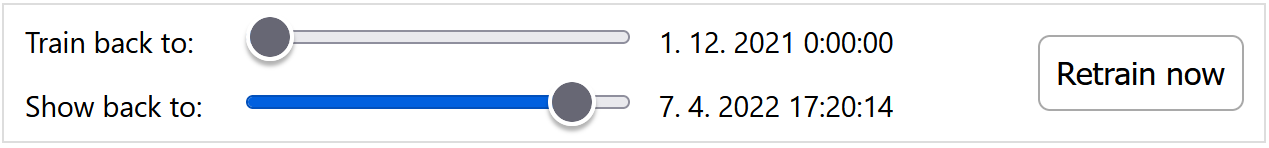
\includegraphics[draft=\draftfig,width=\textwidth]{img/gui/zahlavi.png}
        \caption[Záhlaví GUI]{Záhlaví grafického uživatelského rozhraní systému pro automatické ovládání žaluzie. Umožňuje nastavení intervalu pro zobrazení dat a pro trénování neuronových sítí využívaných pro ovládání žaluzie a spuštění přetrénování na zvolených datech.}
        \label{fig:zahlavi}
    \end{figure}
\section{Stránka Data} \label{sec:data}
    \begin{figure}[h]
        \centering
        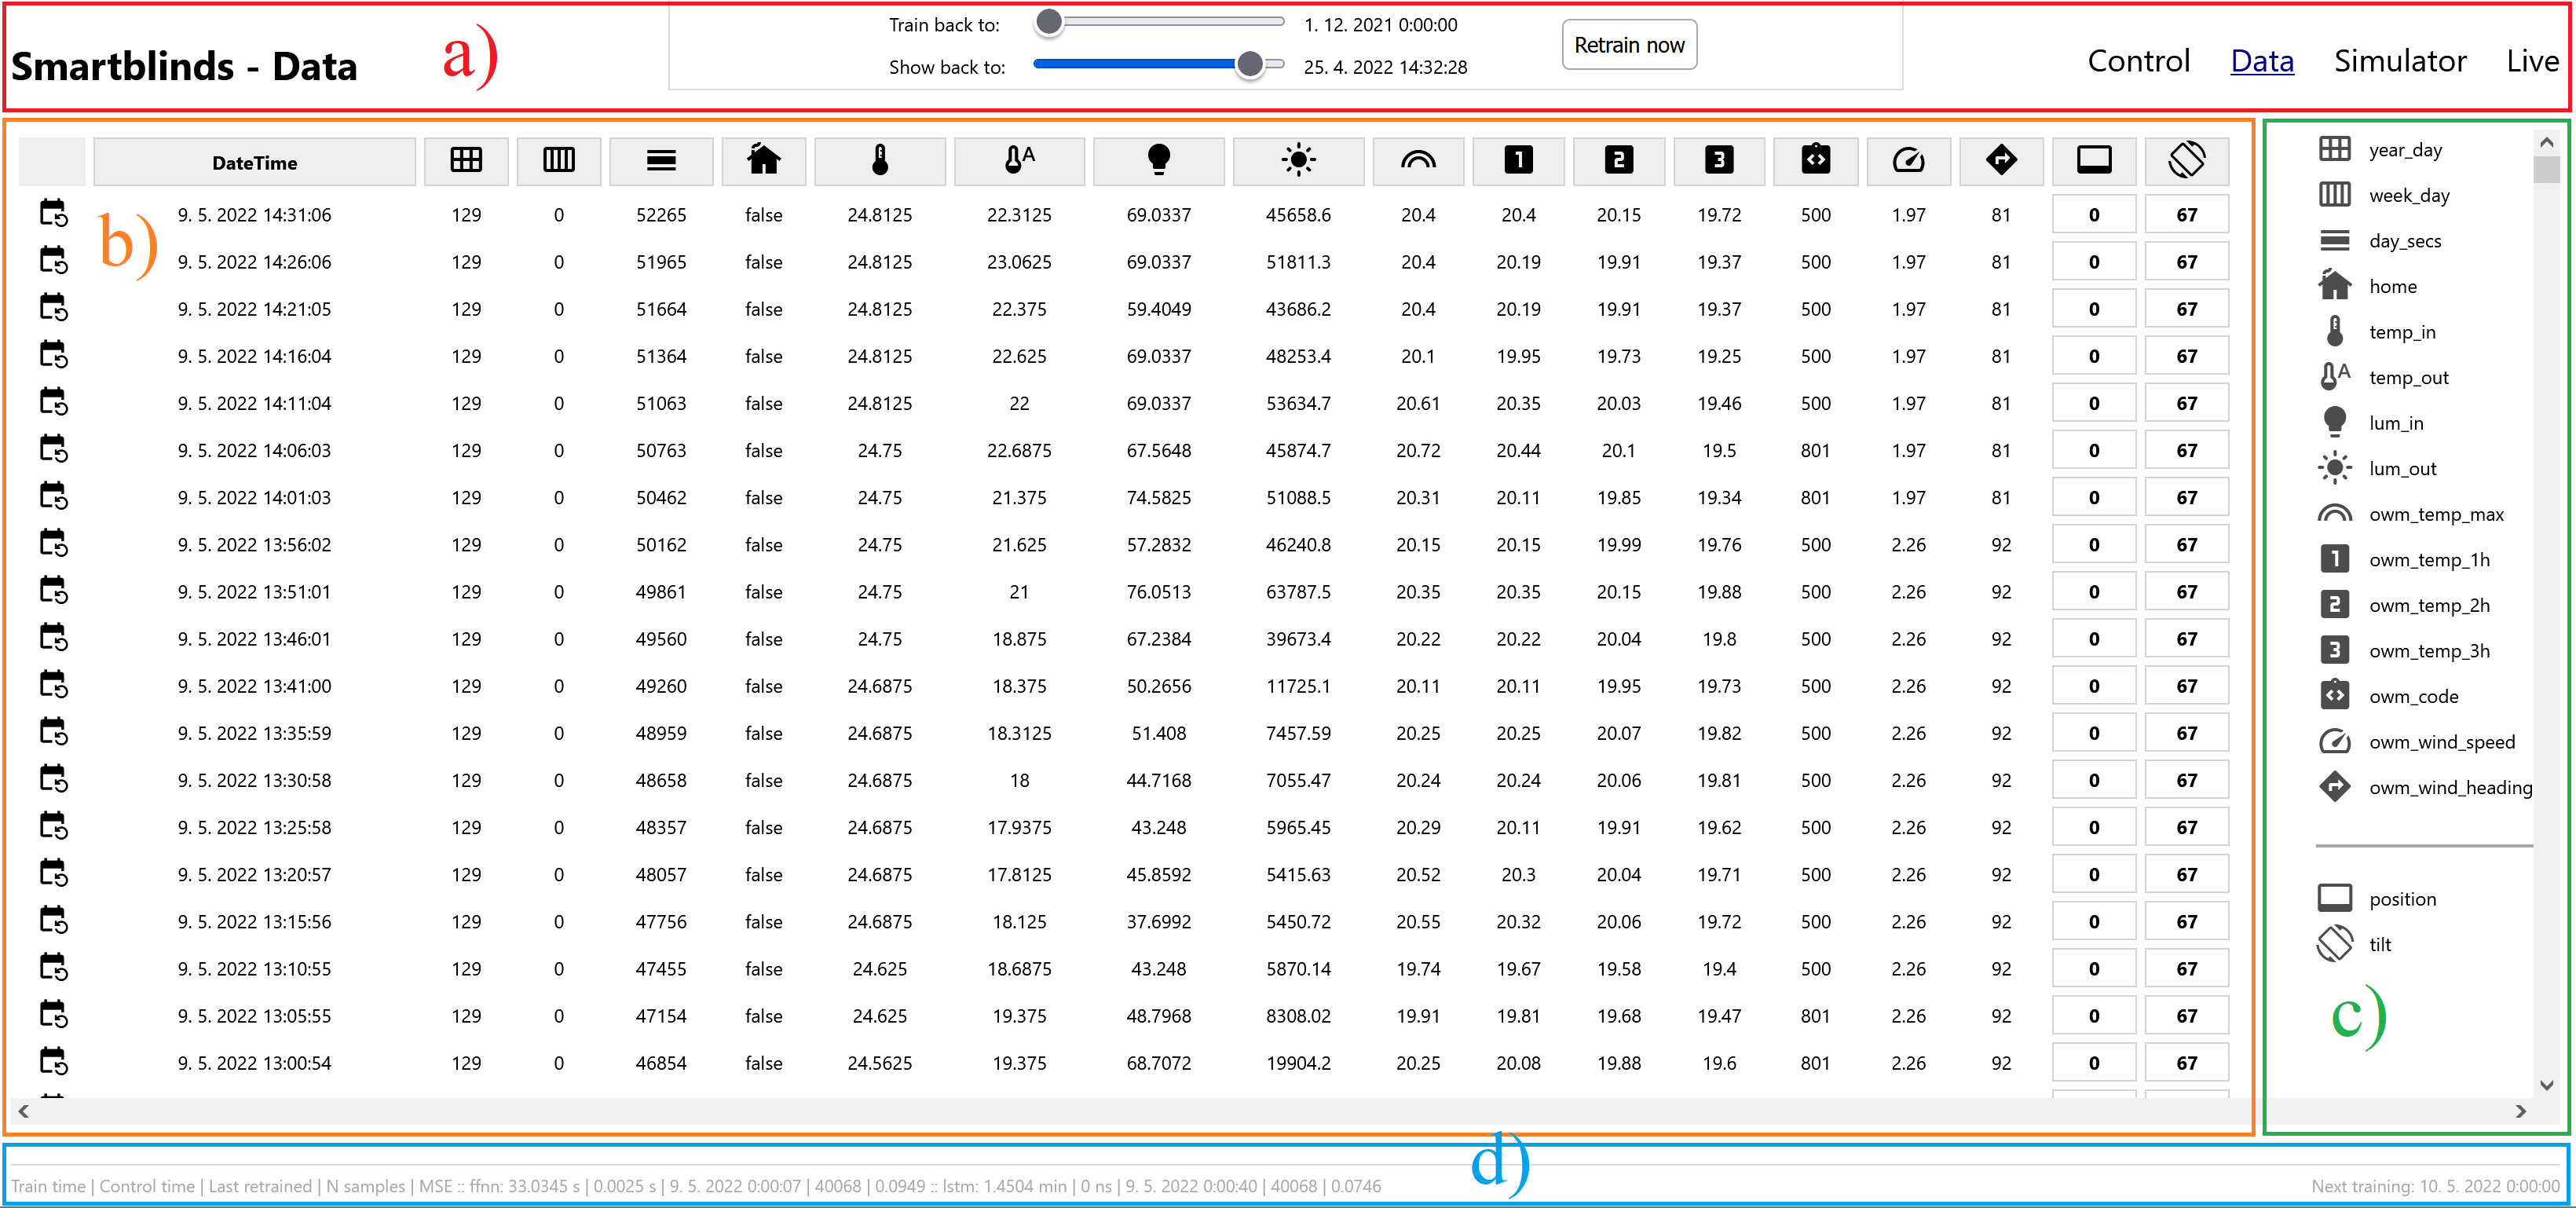
\includegraphics[draft=false,width=\textwidth]{img/gui/data.png}
        \caption[Stránka Data v GUI]{Stránka Data v grafickém uživatelském rozhraní systému pro automatické ovládání žaluzií s vyznačenými částmi pomocí barevných obdélníků \textcolor{guired}{a)} -- \textcolor{guiblue}{d)}}
        \label{fig:data}
    \end{figure}
    Většinu stránky Data (\cref{fig:data}) zaujímá tabulka (\textcolor{guiorange}{b)}), ve které jsou v řádkách uvedeny jednotlivé vzorky naměřených dat s hodnotami všech příznaků a řízení žaluzií uživatelem společně s časem pořízení vzorku. Vlevo od každého řádku je navíc ikona, která reprezentuje příčinu pořízení vzorku: 
\includegraphics[height=0.85\baselineskip]{img/periodic.eps} pro periodické vzorky, 
\includegraphics[height=0.85\baselineskip]{img/event.eps} pro vzorky pořízené na základě změny stavu žaluzie (toto chování je popsáno v \refskl{chap:dataCollection}{kapitole}). Vzorky jsou seřazeny chronologicky od nejmladších k nejstarším a zobrazují se pouze ty, které jsou z časového intervalu daného nastavením v záhlaví aplikace (\textcolor{guired}{a)}, popsáno v úvodu \hyperref[chap:gui]{této kapitoly}). V záhlaví tabulky jsou místo označení příznaků použity ikony, které nezabírají tolik místa. Jejich význam vysvětluje legenda, která je umístěna vpravo od tabulky (\textcolor{guigreen}{c)}). Záhlaví tabulky i legenda zůstávají při rolování tabulkou směrem ke starším datům zafixované v horní části pohledu tak, aby měl uživatel stále přehled o významu hodnot, které sleduje.
    % \begin{figure}
    %     \centering
    %     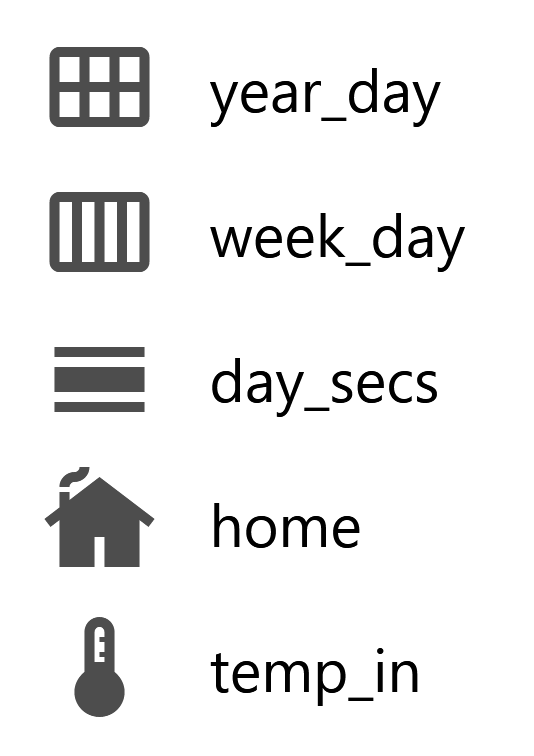
\includegraphics[draft=\draftfig,width=0.22\textwidth]{img/gui/legenda.png}
    %     \caption[Legenda tabulky s daty]{Část legendy tabulky s naměřenými daty v grafickém uživatelském rozhraní systému pro automatické ovládání žaluzií.}
    %     \label{fig:legenda}
    % \end{figure}
\section{Stránka Simulator} \label{sec:sim}
    \begin{figure}[h]
        \centering
        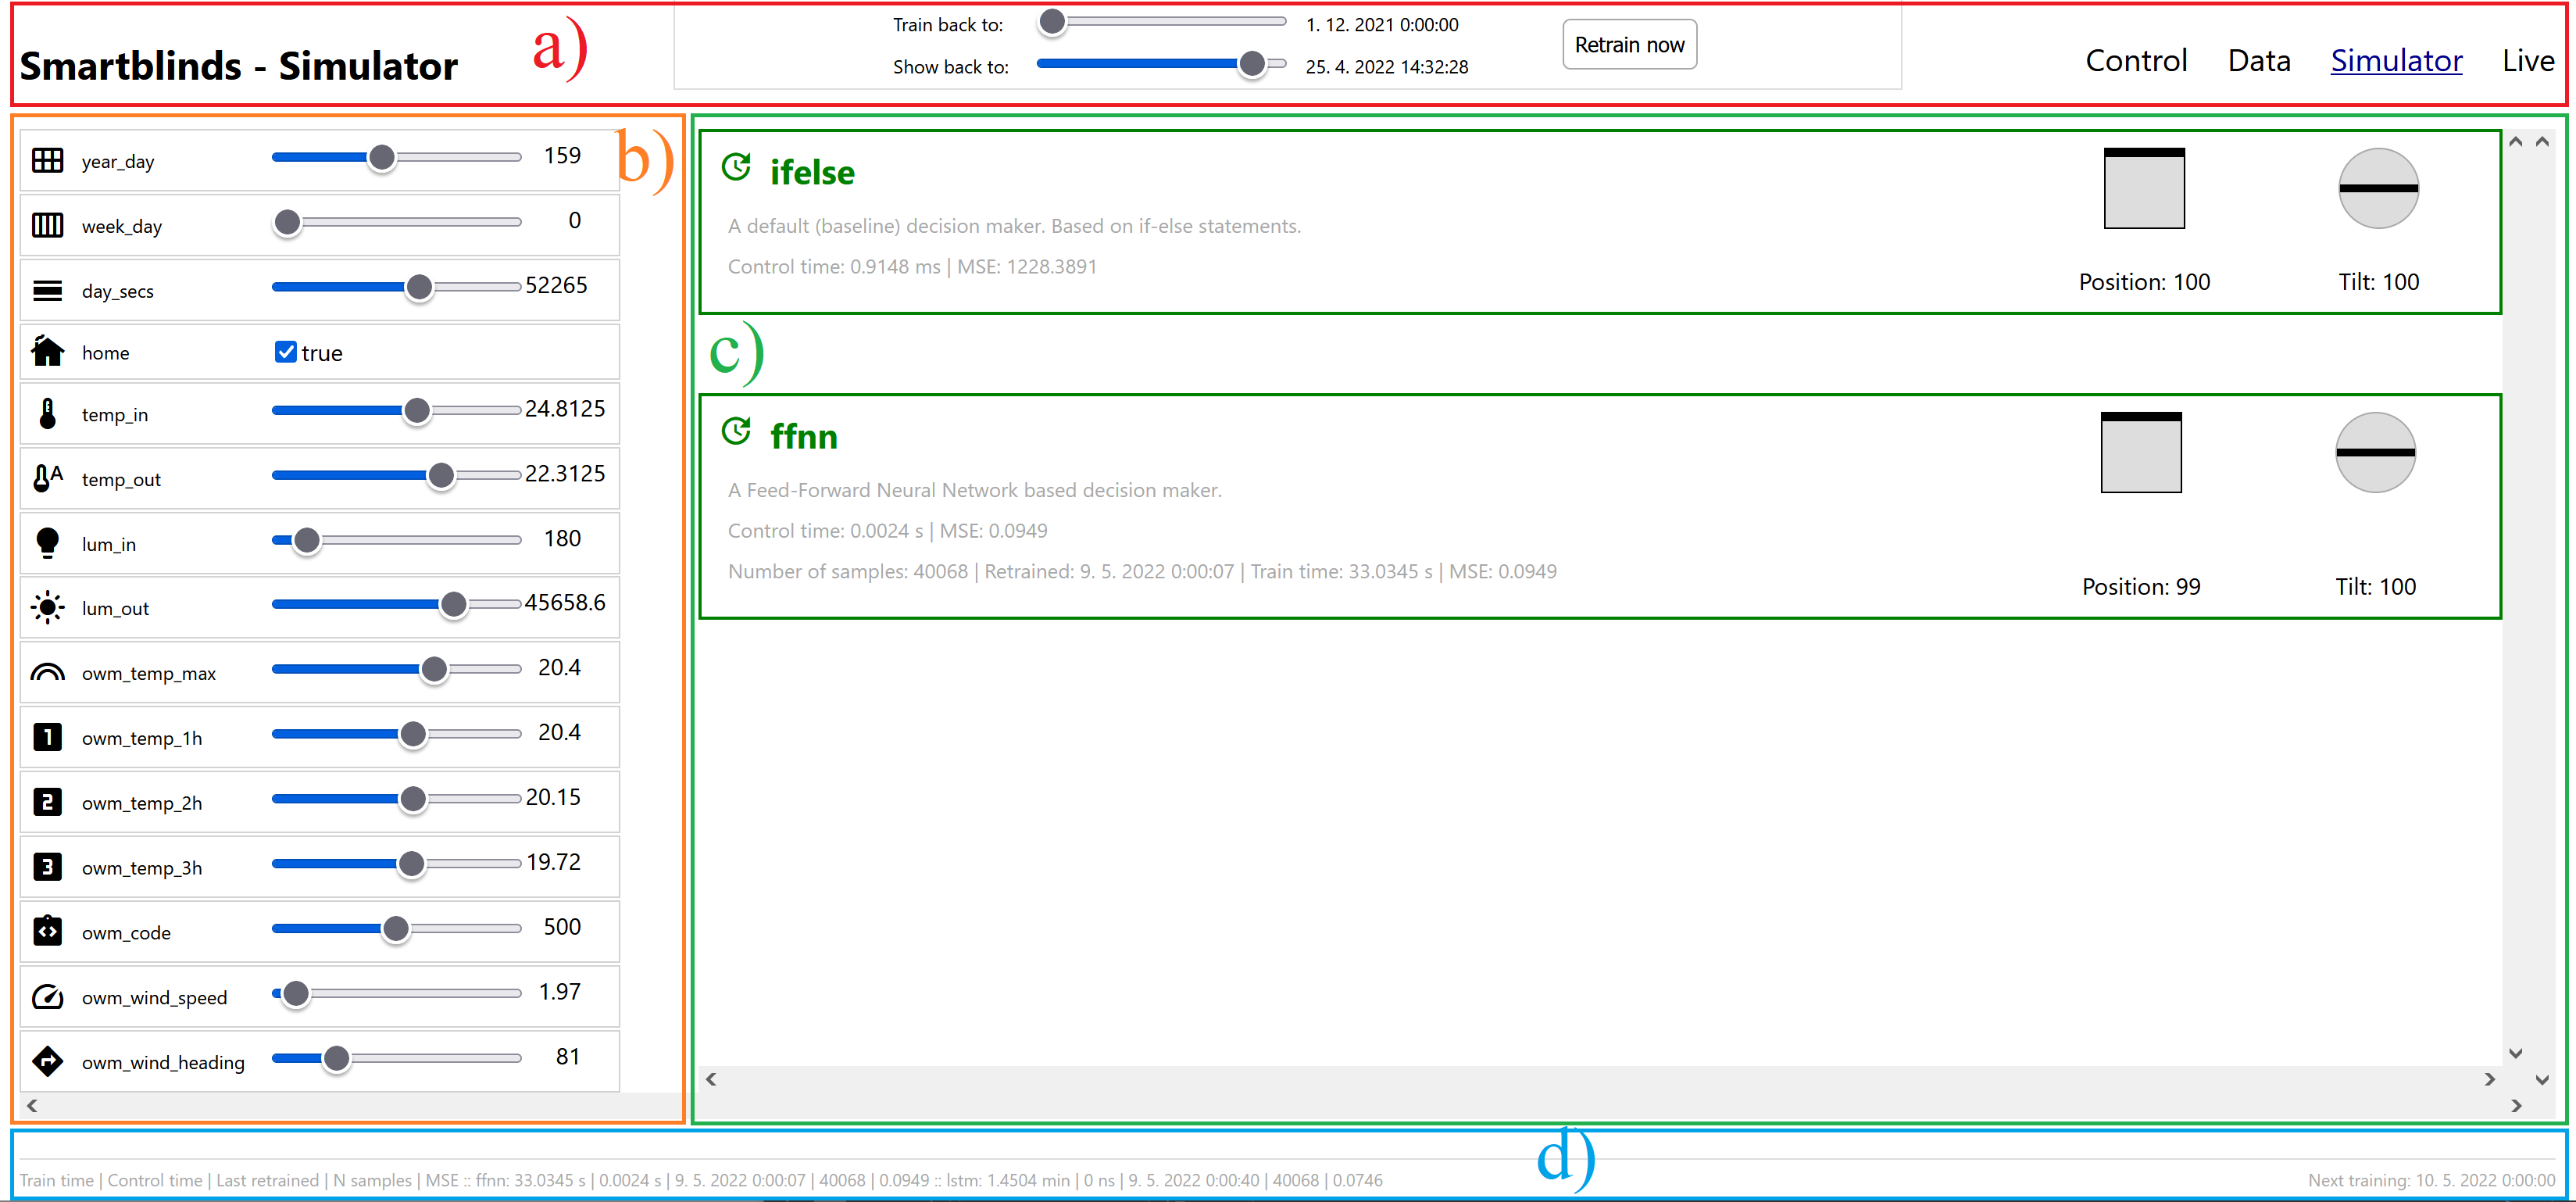
\includegraphics[draft=false,width=\textwidth]{img/gui/simulator.png}
        \caption[Stránka Simulator v GUI]{Stránka Simulator v grafickém uživatelském rozhraní systému pro automatické ovládání žaluzií s vyznačenými částmi pomocí barevných obdélníků \textcolor{guired}{a)} -- \textcolor{guiblue}{d)}}
        \label{fig:simulator}
    \end{figure}
    Tato stránka slouží pro ruční vyhodnocování výstupu regresorů v závislosti na nastavených hodnotách příznaků. Je rozdělena do dvou částí, vlevo je sloupec vstupních prvků (\textcolor{guiorange}{b)}), vpravo pak rámce jednotlivých regresorů s jejich výstupem a jeho jednoduchou vizualizací (\textcolor{guigreen}{c)}). Výška vytažení žaluzie (Position) je reprezentována částečným vybarvením obdélníku shora, úhel naklopení lamel (Tilt) pak rotací čáry uvnitř kruhu (příklad je na \refskl{fig:vizualizace}{obrázku}).
    
    Vzhledem k povaze vstupních prvků (\textcolor{guiorange}{b)}), pomocí kterých je možné zadat hodnoty pouze v jednom časovém okamžiku, se vyhodnocuje výstup pouze regresoru If-else a FFNN, regresor LSTM totiž vyžaduje hodnoty příznaků ne z jednoho, ale z 64 okamžiků, což by vyžadovalo složitější způsob zadávání.
    
    Při každé změně vstupu se pro každý sledovaný regresor odešle požadavek na endpoint \code{ep\_control} backendu systému (\cref{sec:tornado}), v odpovědi se vrátí výstup regresoru, který je poté zobrazen.
    \begin{figure}
        \centering
        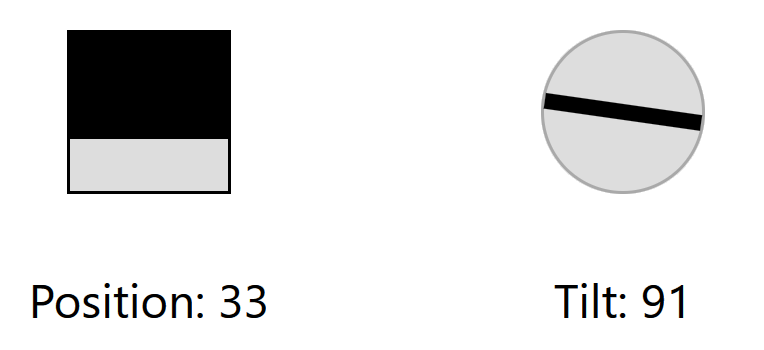
\includegraphics[draft=\draftfig,width=0.44\textwidth]{img/gui/vizualizace.png}
        \caption[Vizualizace výstupu regresoru]{Příklad vizualizace výstupu regresoru v úloze automatického ovládání žaluzie na základě 15 příznaků.}
        \label{fig:vizualizace}
    \end{figure}
\section{Stránka Control} \label{sec:control}
    \begin{figure}[h]
        \centering
        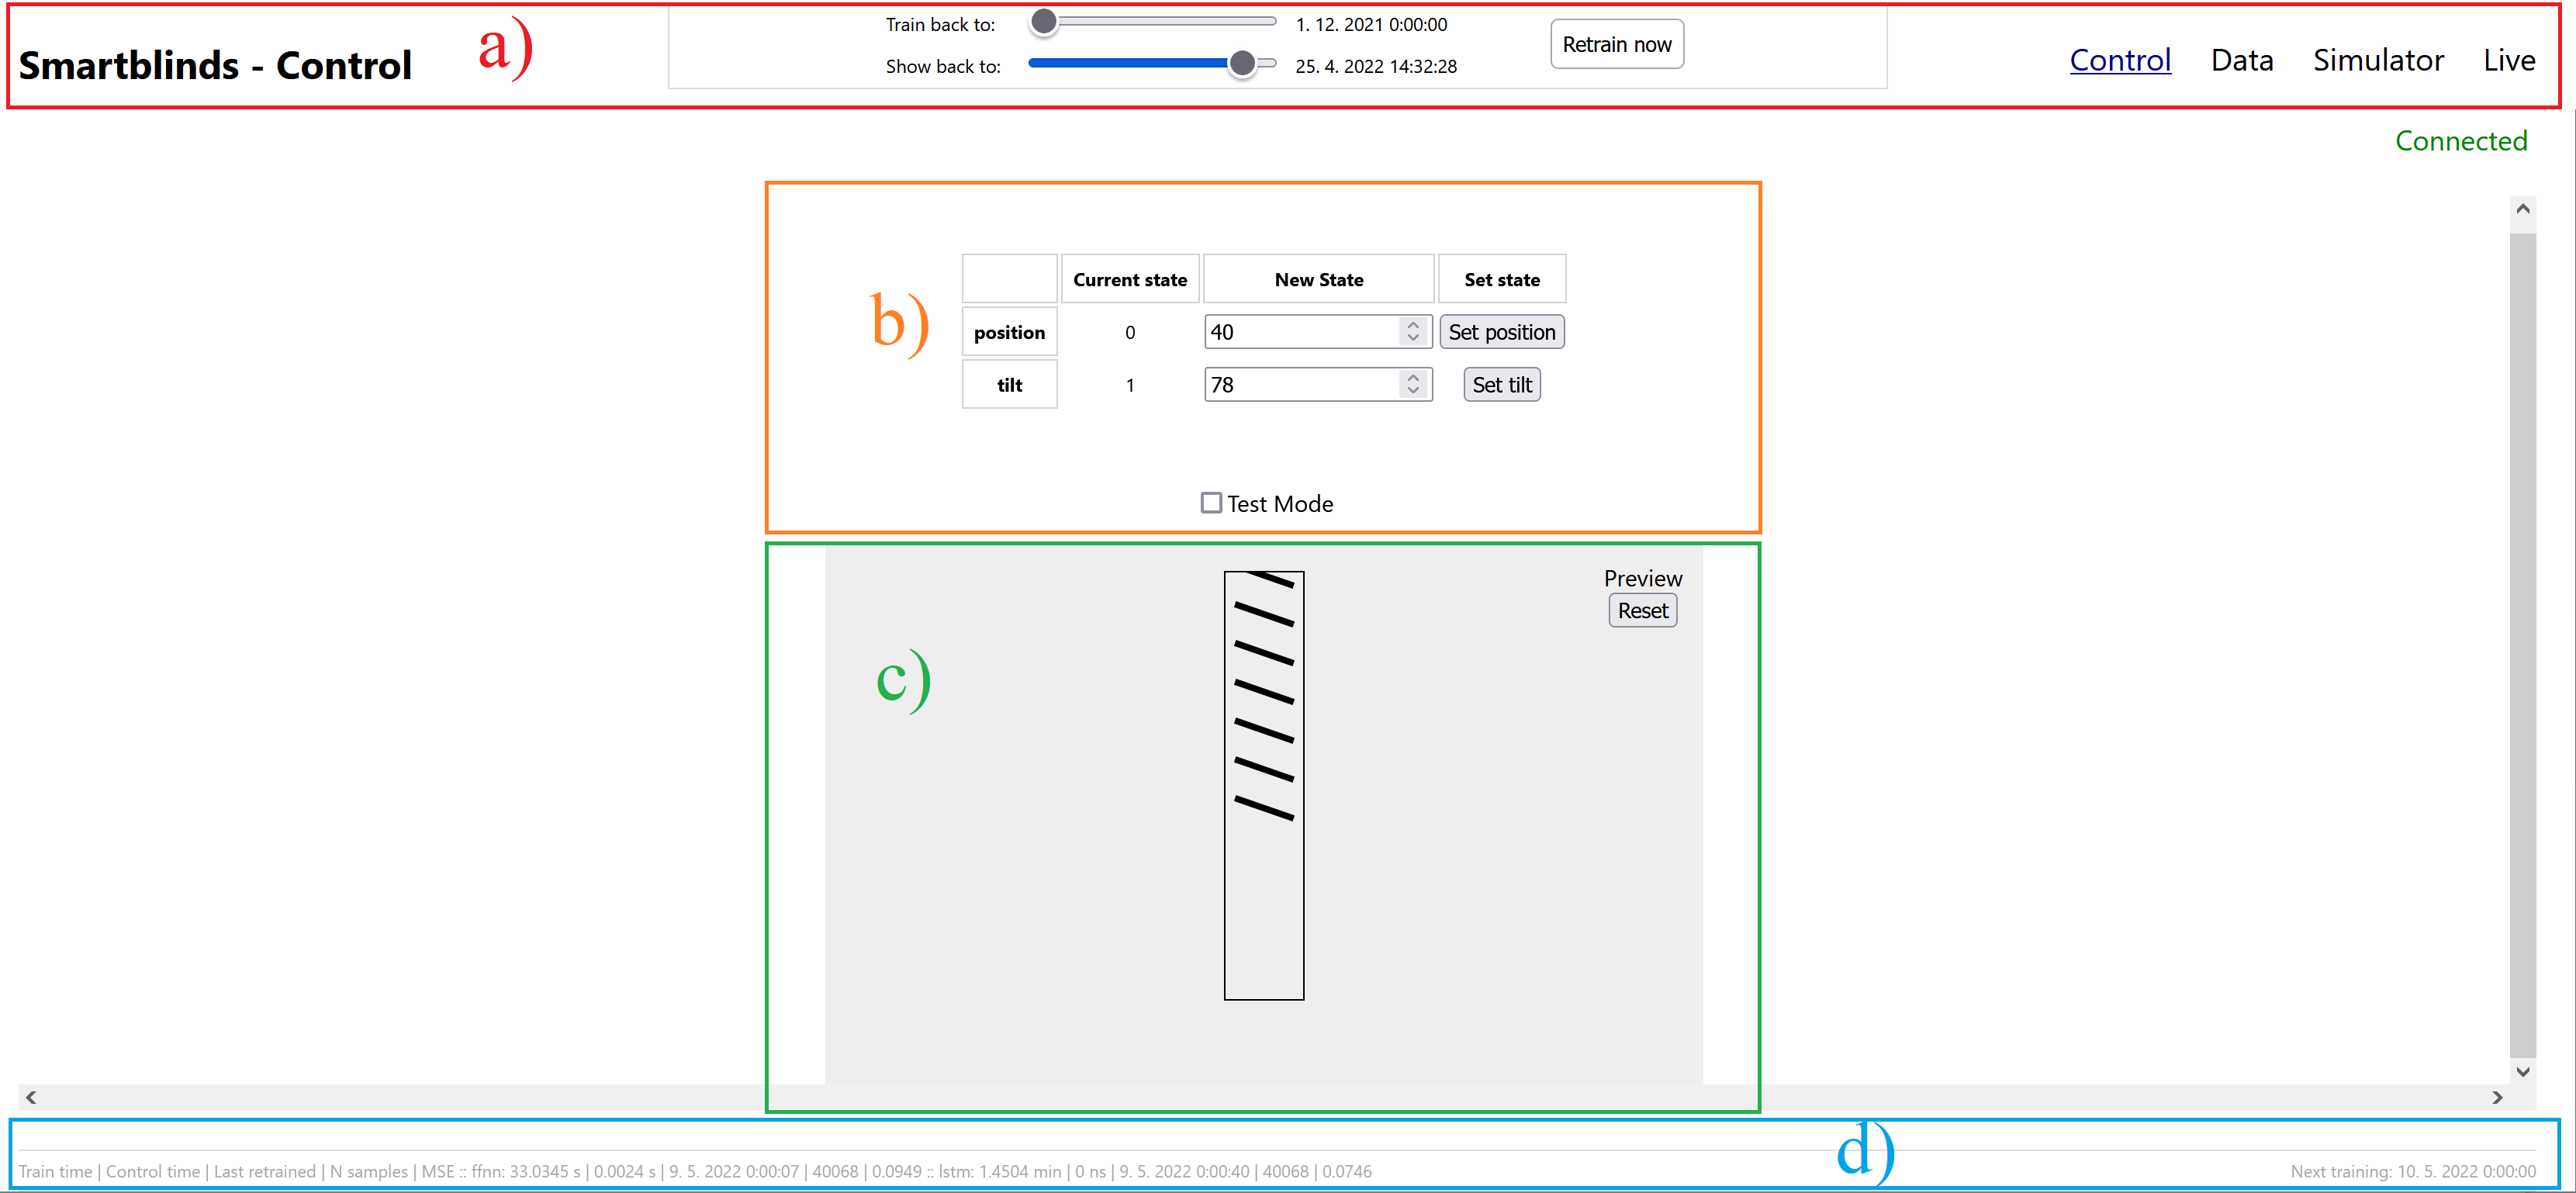
\includegraphics[draft=false,width=\textwidth]{img/gui/control.png}
        \caption[Stránka Control v GUI]{Stránka Control v grafickém uživatelském rozhraní systému pro automatické ovládání žaluzií s vyznačenými částmi pomocí barevných obdélníků \textcolor{guired}{a)} -- \textcolor{guiblue}{d)}}
        \label{fig:control}
    \end{figure}
    Další stránkou v \acrshort{gui} je Control, která slouží k zobrazení aktuálního stavu žaluzie a k jeho ruční změně. Skládá se ze dvou hlavních částí uspořádaných pod sebou - tabulky se stavy žaluzie (nahoře, \textcolor{guiorange}{b)}) a vizualizace (dole, \textcolor{guigreen}{c)}).

    Tabulka (\textcolor{guiorange}{b)}) má tři sloupce, v prvním z nich se zobrazuje aktuální stav, ve druhém jsou pole pro nastavení nového stavu a ve třetím tlačítka pro odeslání požadavku na změnu stavu. Každý řádek je pro jednu stavovou proměnnou žaluzie.

    Vizualizace (\textcolor{guigreen}{c)}) zobrazuje žaluzii v řezu. Počet lamel a vzdálenost spodní lamely od okraje odráží výšku vytažení žaluzie, jejich odchylka od vodorovné osy pak odpovídá náklonu lamel skutečné žaluzie. Při změně hodnot v tabulce se vizualizace přepne do režimu náhledu, kdy je možné sledovat, jak by skutečná žaluzie vypadala, pokud by se odeslaly hodnoty nastavené v tabulce. Uživatele o tom informuje text \emph{Preview} v pravém horním rohu vizualizace. Tlačítkem \emph{Reset}, nacházejícím se tamtéž, je možné tento režim opustit a vizualizace pak bude opět zobrazovat aktuální stav žaluzie. Vizualizace je psána ve značkovacím jazyce pro dvourozměrnou vektorovou grafiku SVG (\cite{w3c:svg}).

    Mezi tabulkou a vizualizací je navíc ještě zaškrtávací pole \emph{Test Mode}, které umožňuje aktivovat nebo deaktivovat testovací režim při sběru dat, který se využívá při vývoji, aby databáze neobsahovala data vzniklá na základě falešných událostí.

    Pro získávání aktuálního stavu a nastavení nového se používá spojení s backendem (\cref{sec:tornado}) pomocí protokolu WebSockets na jeho endpointu \code{ws}. Po připojení je každých 15~{s} do webového prohlížeče uživatele \acrshort{gui} doručován aktuální stav žaluzie ve zprávách ve formátu JSON a stejným způsobem se odesílá požadavek na jeho změnu. V pravém horním rohu stránky je indikátor spojení pomocí protokolu WebSockets.
\section{Stránka Live} \label{sec:live}
    \begin{figure}[h]
        \centering
        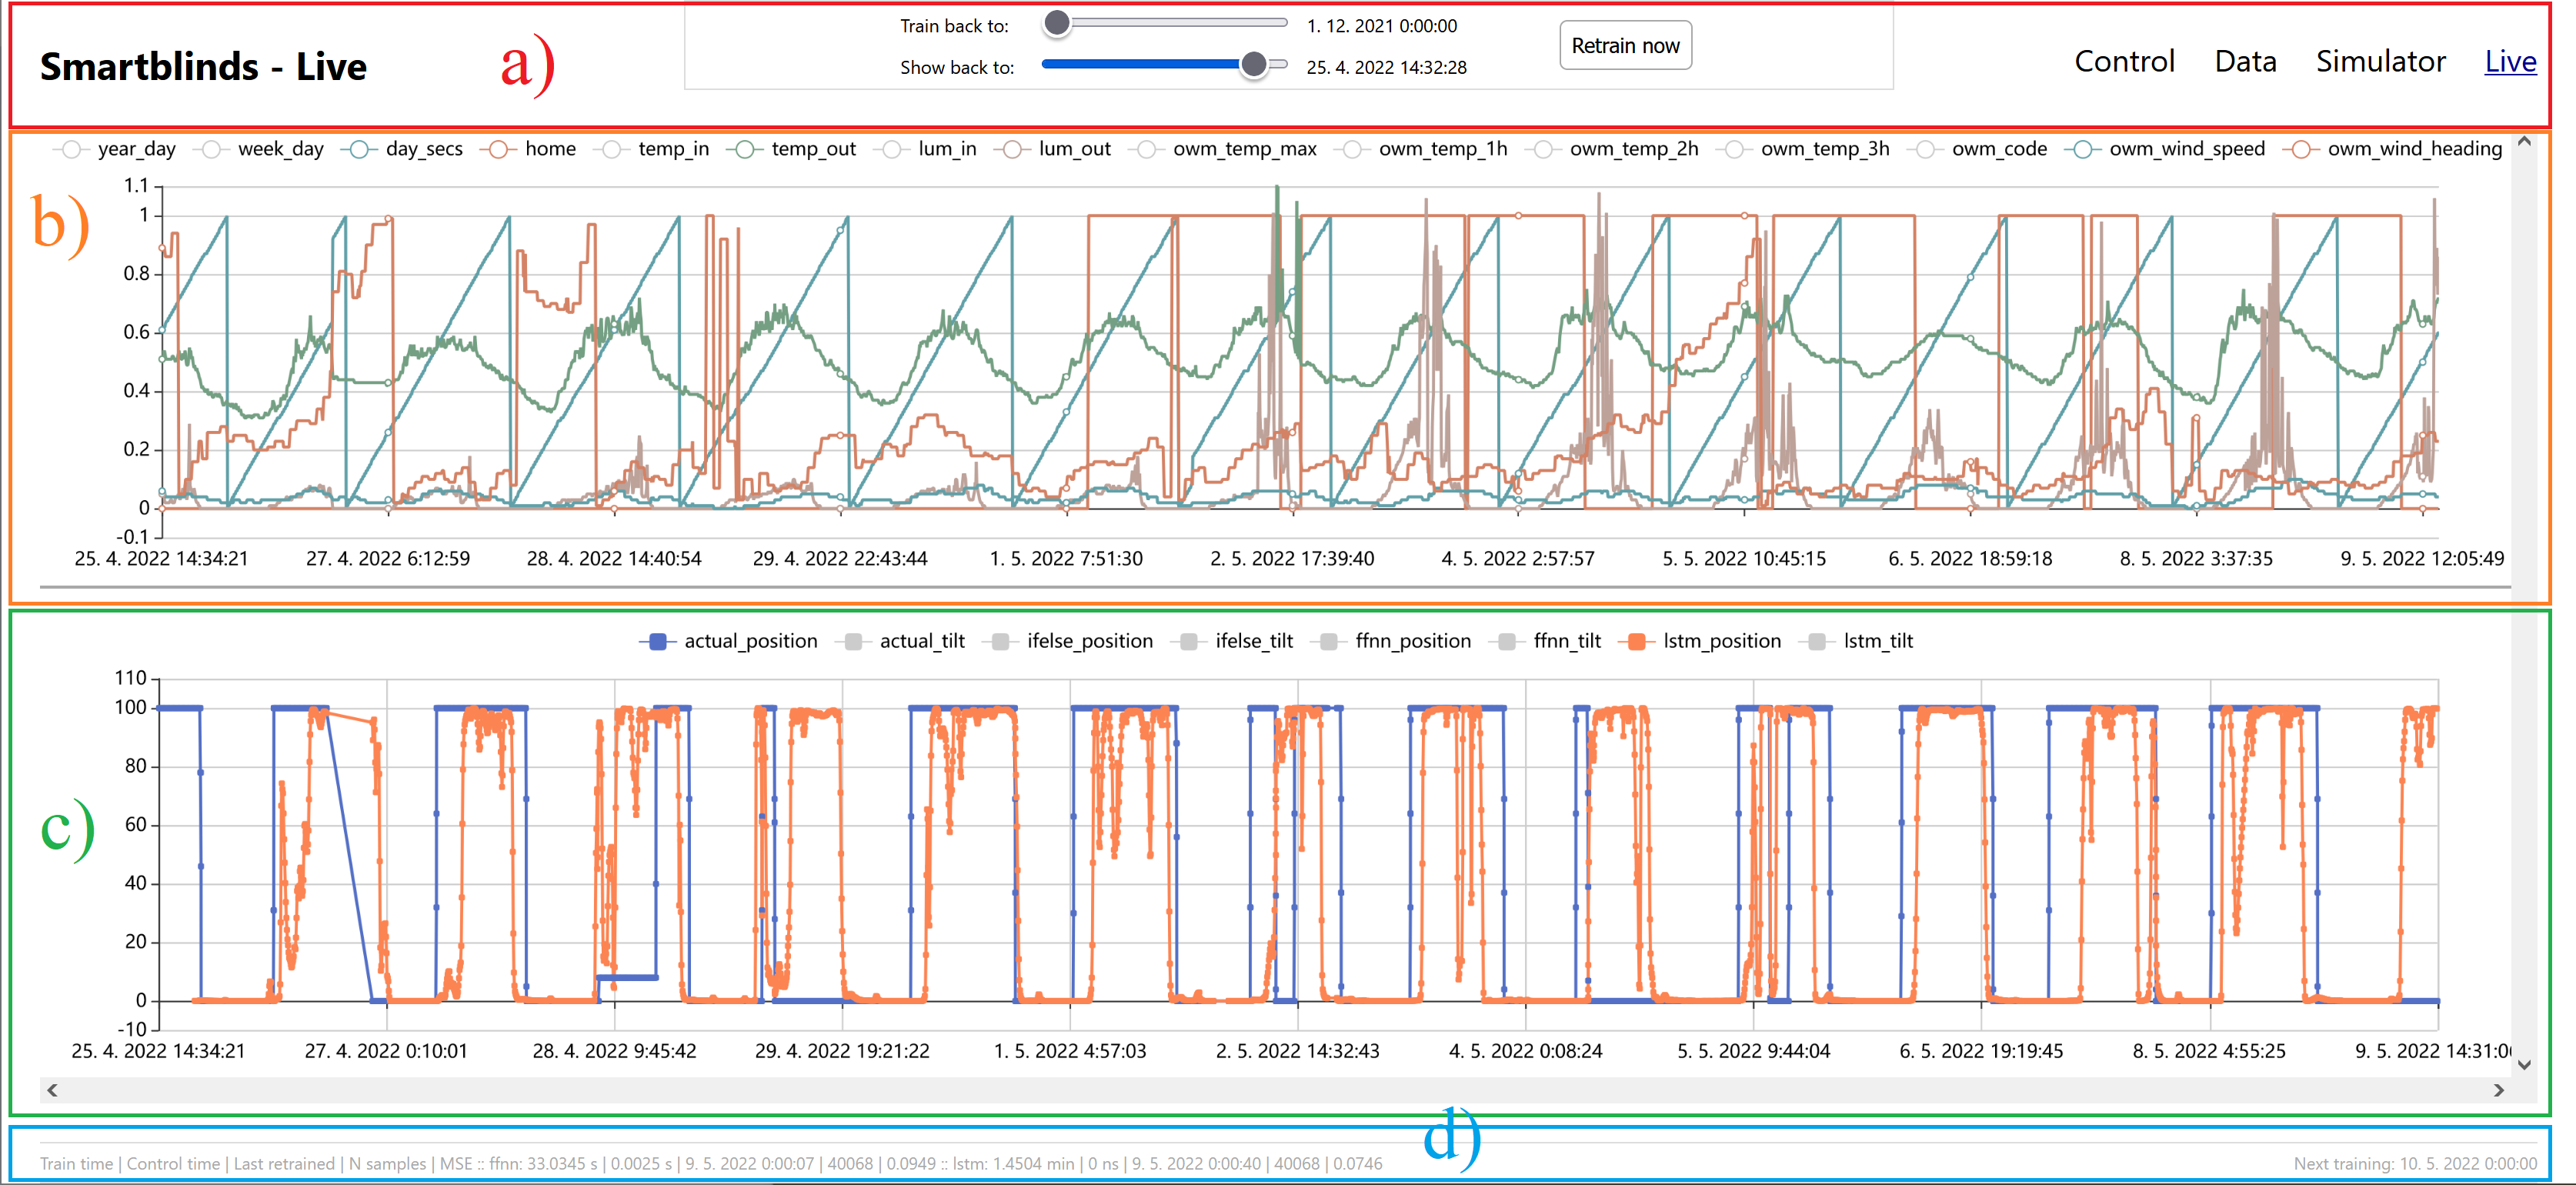
\includegraphics[draft=false,width=\textwidth]{img/gui/Live.png}
        \caption[Stránka Live v GUI]{Stránka Live v grafickém uživatelském rozhraní systému pro automatické ovládání žaluzií s vyznačenými částmi pomocí barevných obdélníků \textcolor{guired}{a)} -- \textcolor{guiblue}{d)}}
        \label{fig:live}
    \end{figure}
    Poslední ze 4 stránek \acrshort{gui} je stránka Live, která slouží k živému vyhodnocování řízení doporučeného jednotlivými regresory na reálných datech. Skládá se ze dvou grafů uspořádaných pod sebou. V horním grafu ((\textcolor{guiorange}{b)}) jsou zobrazena naměřená data, v dolním (\textcolor{guigreen}{c)}) pak řízení žaluzie (manuální řízení i doporučené řízení regresorů). Nad každým z grafů se nachází interaktivní legenda, která umožňuje skrývat některé linie v grafu pro větší přehlednost podle požadavků uživatele \acrshort{gui}. Kurzorem myši lze sledovat konkrétní hodnoty všech veličin v grafu v okamžiku daném jeho polohou.

    Data zobrazovaná v grafech se získávají pomocí 2 požadavků zasílaných na endpointy backendu (\cref{sec:tornado}). Naměřená data se přenáší vždy všechna na základě požadavku na \code{ep\_data} při prvním načítání aplikace, predikce regresorů kromě okamžiku prvního načtení aplikace také vždy při změně časového intervalu pro zobrazení dat v záhlaví aplikace (popsáno v úvodu \hyperref[chap:gui]{této kapitoly}). Oba grafy ale vždy zobrazují pouze data z časového intervalu daného nastavením v záhlaví stránky (\textcolor{guired}{a)}, \emph{Show back to:}).